\begin{frame}
  \frametitle{1D Chain of Atoms}
  % \begin{columns}
  %   \begin{column}
      
  %   \end{column}
  % \end{columns}
  \begin{center}
    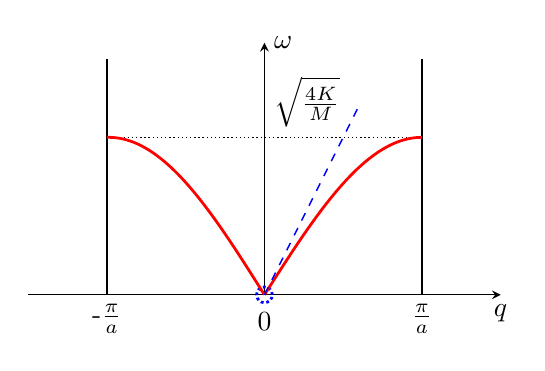
\begin{tikzpicture}
      [scale=2.0]
      \draw[->, >=stealth] (-1.5, 0.0) -- (1.5, 0.0) node[below] {$q$};
      \draw[->, >=stealth] (0.0, 0.0) -- (0.0, 1.6) node[right] {$\omega$};
      \node[below=3pt] at (0, 0) {0};

      \draw[line width=0.5pt] (1.0, 0.0) -- (1.0, 1.5);
      \draw[line width=0.5pt] (-1.0, 0.0) -- (-1.0, 1.5);
      \draw[line width=0.5pt, densely dotted] (-1.0, 1.0) -- (1.0, 1.0);
      \draw[blue, line width=1pt, densely dotted] (0.0, 0.0) circle (0.05);

      \node[below, align=left] at (1.0, 0.0) {${\pi\over a}$};
      \node[below, align=right] at (-1.0, 0.0) {-${\pi\over a}$};
      \node[right, anchor=south west] at (0.0, 1.0) {$\sqrt{4K\over M}$};

      \draw[line width=1.0pt, color=red, domain=0:1.0, solid] plot[samples=300]
      (\x, {sin(\x r * pi / 2)});
      \draw[line width=1.0pt, color=red, domain=-1:.0, solid] plot[samples=300]
      (\x, {-sin(\x r * pi / 2 \x)});
      \draw[line width=0.5pt, color=blue, domain=0:.6, dashed] plot[samples=300]
      (\x, {\x * 2.});
    \end{tikzpicture}
  \end{center}

  \begin{center}
    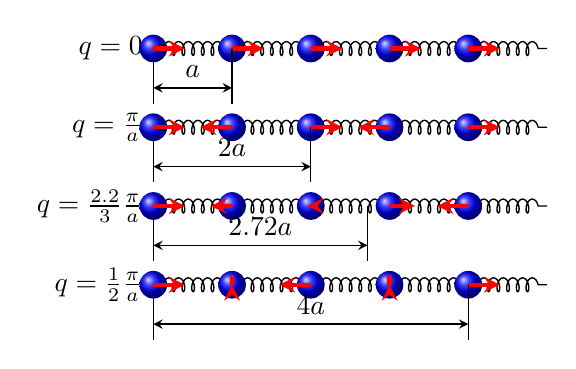
\begin{tikzpicture}
      [
      spring/.style={
        line width=0.5pt,
        decorate,
        decoration={
            coil,
            amplitude=2.5,
            segment length=3.5,
          }
        },
      ]
      \foreach \y/\q/\lab in {0/0.0/0, -1/1.0/\frac{\pi}{a}, -2/0.7333333333/\frac{2.2}{3}{\pi\over a}, -3/0.5/{1\over 2}\frac{\pi}{a}}
      {
        \node[left=0.3, align=right] at (0.0, \y) {$q=\lab$};
        \draw[line width=0.5pt] (0.0, \y) -- ++(0.0,-0.7);

        \foreach \x in {0,1,...,4}{
            % draw the spring
            \ifthenelse{\x < 4}
            {
              \draw[spring, draw=black] (\x, \y) -- ++(1, 0);
            }{}
            % draw the atoms
            \shade[ball color=blue] (\x, \y) circle (5pt);

            \pgfmathparse{0.4*cos(\q*pi*\x r)}
            \let \A = \pgfmathresult
            \draw[->, >=stealth, line width=1.5pt, draw=red] (\x, \y) -- ++(\A, 0.0);
        }
      }
      \draw[line width=0.5pt] (1.0, 0) -- ++(0.0,-0.7);
      \draw[line width=0.5pt] (2.0, -1) -- ++(0.0,-0.7);
      \draw[line width=0.5pt] (2.72, -2) -- ++(0.0,-0.7);
      \draw[line width=0.5pt] (4.0, -3) -- ++(0.0,-0.7);

      \draw[line width=0.5pt, <->, >=stealth] (0.0, -0.5) -- node[pos=0.5, anchor=south] {$a$} (1.0,-0.5);
      \draw[line width=0.5pt, <->, >=stealth] (0.0, -1.5) -- node[pos=0.5, anchor=south] {$2a$} (2.0, -1.5);
      \draw[line width=0.5pt, <->, >=stealth] (0.0, -2.5) -- node[pos=0.5, anchor=south] {$2.72a$} (2.72,-2.5);
      \draw[line width=0.5pt, <->, >=stealth] (0.0, -3.5) -- node[pos=0.5, anchor=south] {$4a$} (4.0,-3.5);

      
    \end{tikzpicture}
  \end{center}
\end{frame}
%%% Local Variables:
%%% mode: latex
%%% TeX-master: t
%%% End:
